\documentclass{article}

\usepackage{amsmath}
\usepackage{graphicx}
\usepackage{caption}
\usepackage{subcaption}
\usepackage{color}
\usepackage{listings}
\usepackage{booktabs}
\usepackage{forest}

\title{
	\underline{CS6370: Natural Language Processing}\\
	\textbf{Spell Check Assignment Report}\\
	Indian Institute of Technology Madras
}
\author{
	\textbf{Chinni Chaitanya, EE13B072}\\
	\texttt{ee13b072@smail.iitm.ac.in}	
	\and
	\textbf{Venkatesh Maligireddy, EE13B041}\\
	\texttt{ee13b041@smail.iitm.ac.in}
	\and
	\textbf{Swaroop Kotni, EE13B030}\\
	\texttt{ee13b030@smail.iitm.ac.in}
	\and
	\textbf{Pronnoy Noel, EE13B029}\\
	\texttt{ee13b029@smail.iitm.ac.in}
}

\begin{document}
	\pagenumbering{gobble}
	\maketitle
	\newpage
	
	\pagenumbering{roman}
	\tableofcontents
	\newpage
	
	\pagenumbering{arabic}
	\section{Introduction}
		This assignment attempts to implement \textit{spell checker and correction} programs for text, which will correct the erroneous word\footnote{In phrases and sentences, the erroneous word need not be misspelled but might be contextually incorrect.} present in it. The assignment is categorized into the following three parts,
		\begin{description}
			\item[$\bullet$] \textbf{Word checker}, a program which checks and corrects standalone erroneous words\footnote{The word given might be correct word also.}.
			\item[$\bullet$] \textbf{Phrase checker}, a program which examines phrases and corrects the erroneous words. We assume \textit{phrases} contain about 5 words.
			\item[$\bullet$] \textbf{Sentence checker}, a program which examines sentences and corrects the erroneous words. We assume \textit{sentences} contain about 30 words.
		\end{description}
		In all the three cases, we assume that there is only \textbf{one} erroneous word.
		\subsection{Directory structure}
			The submission contains the following folder structure,\\
			\texttt{
				/src\\
				....bayesian.py\\
				....editex.py\\
				....stringTokenize.py\\
				....trie.py\\
				....phrase\_check.py\\
				....word\_check.py\\
				README\\
				Report\_Team10.pdf
			}
		
	\section{Data generation}
		\subsection{Corpa used for data generation}
			We have used \textit{brown corpus} and \textit{american-english} dictionary available in Linux and generated all the required data (confusion sets, context words frequencies etc.,)
			
	\section{Word checker}
		The \textit{word checker} aims to implement a program to inspect the standalone erroneous word given as input, and come up with a set of possible candidates with their probability of correctness and ranking. The probability of each word is calculated both \textbf{\textit{statistically (Bayesian probability)}} \cite{bayesian} as well as \textbf{\textit{phonetically (editex)}} \cite{phonetic}. All the main ideas regarding ranking and probabilities are taken from \cite{bayesian} and \cite{phonetic}.\\
		This whole implementation can be broken into the following four sub-tasks,
		\begin{description}
			\item[$\bullet$ Task-1] Generation of candidate set for the given erroneous word
			\item[$\bullet$ Task-2] Calculate the Bayesian probability for each word in the candidate set
			\item[$\bullet$ Task-3] Calculate the phonetic probability for each word in the candidate set
			\item[$\bullet$ Task-4] Combine both Bayesian and phonetic probabilities and rank the words in the candidate set
		\end{description}
		
		\subsection{Generation of candidates}
			The aim of this task is to generate the set of candidate words or the candidate set for the erroneous word given. A crude way to do this is to generate all possible strings for the given erroneous word by adding, deleting, substituting and reversing the letters in the given word and check whether that string exists in the dictionary. This works, but is computationally intensive. Hence, we need to intelligently store the words in the dictionary such that, the search doesn't take much time. Instead of the additional step to generate the possible strings and check if they exist in the dictionary, we could intelligently fetch the words from the dictionary itself by some measure. One such measure is \textit{Levenshtein distance}. The following sub-sections attempt to address these ideas. 
			\subsubsection{Levenshtein distance}
				Levenshtein Distance between two strings is given by the minimum number of edits, substitution, insertion, deletion required to change one string to another. We have implemented the \textit{dynamic programming} approach to calculate the Levenshtein distance between the candidates and the incorrect word.
				\begin{description}
					\item[$\bullet$] Levenshtein distance follows the triangular inequality. That is,\\
					$d(x,y) + d(y,z) \geq d(x,z)$.
					\item[$\bullet$] It is commutative. That is,\\ $d(x,y) = d(y,x)$.
					\item[$\bullet$] All the values in the last row are greater than the Levenshtein distance except the last value (used for searching in \textit{Trie}).
				\end{description}
				
			\subsubsection{Burkhard-Keller Trees or BK-Trees}
				BK-Tree is a tree data structure used for spell checking based on the Levenshtein distance between two words. All the words in the dictionary are iterated and inserted one by one into the tree. The insertion goes as follows,\\
				The first word of dictionary becomes the root word of tree with an associated dictionary to it. Then to insert the next word, the Levenshtein distance is calculated between root and current word and the current word is inserted at the \textit{key} equal to the levenshtein distance in the root dictionary. If that key already exists, the same process is repeated for the word at that Levenshtein distance. The triangular inequality of the levenshtein distance is used while searching in the bk-tree to get the candidate words.
			
			\subsubsection{Trie structure}
				This is also a tree data structure. The root word is null. Each node is associated with a children dictionary. Now to insert the word, the first letter of the word is checked if present in the children of the root node. If not present, it is created. If present, it will go to the next character in the word and repeats the same with the children dictionary of the correct letter.\\
				The property of the levenshtein distance that the last row of the matrix have all values except the last value greater than the levenshtein distance is used to search in the trie to get the candidates.

				\begin{minipage}{\linewidth}
					\begin{center}
 						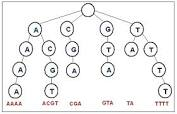
\includegraphics[width=\linewidth]{trie}
 	 					\captionof{figure}{Trie data structure sample}
	  					\label{fig:trie_fig}
					\end{center}
				\end{minipage}\\				
				
		\subsection{Ranking the candidates statistically}
			\subsubsection{Bayesian probability}
				Given the typo \textit{t}, the possible candidates ($c_{i}$) were generated from the Trie data structure which was generated from the dictionary. Now the candidates are ranked based on posterior probability score $P(c|t)$, where \textit{c} is the candidate word
Using the Bayesian rule the probability that the suggested correct word \textit{c}, produces the typo \textit{c} is given by,
				\begin{equation*}
					P(c|t) = P(t|c) \times \frac{P(c)}{P(t)}
				\end{equation*}
				Each candidate correction, is scored by $Pr(c) \times Pr(t|c)$, and then normalized by the sum of the scores for all proposed candidates. The probability $P(t)$ cancels out during normalization.\\
				The frequency of the correct word, $P(c)$ is obtained form the word frequency list which are generated by files from,\\ 
				\texttt{http://opus.lingfil.uu.se/OpenSubtitles2016.php}\\
				For smoothing purposes the frequency of \textit{c} is modified to,
				\begin{equation*}
					P'(c) = \frac{N \times P(c) + 0.5}{N}
				\end{equation*}
				where $N$ is the total number of words in the corpus.
				\subsubsection{Computing $P(t|c)$}
					The conditional probabilities $P(t|c)$, are computed from the four confusion matrices namely deletion, insertion, substitution and reversal,
					
					$
					P(t|c) = 
						\left\{	
							\begin{matrix}
								\frac{del[c_{p-1}, c_{p}]}{chars[c_{p-1}, c_{p}]}, \> if \> deletion	\\
								\frac{add[c_{p-1}, t_{p}]}{chars[c_{p-1}]}, \> if \> insertion \\
								\frac{sub[t_{p}, c_{p}]}{chars[c_{p}]}, \> if \> substitution \\
								\frac{rev[c_{p}, c_{p+1}]}{chars[c_{p}, c_{p+1}]}, \> if \> reversal
							\end{matrix}
						\right.
					$
				\subsubsection{Generating single occurrences}
					We generate the single occurrences by parsing every word in the corpus and counting the number of times a character has occurred in the corpus.
				\subsubsection{Generating co-occurrences}
					Similarly for character co-occurrences we parse every word of the corpus and search for a pattern of consecutive characters (say $x, y$). 
For example consider \textit{ae}, we search in the whole corpus for occurrence of the pattern \textit{ae} and the number of occurrences of \textit{ae} gives the co-occurrences of \textit{ae}. Similarly we find the pattern for all the possible co-occurrences. \\
					The confusion matrices are pre-computed from the training corpus 1988 AP corpus.\\

			\medskip
					
			From the list of candidates we receive from the Trie data structure, we use Levenshtein edit distance to identify the deletions, substitutions etc for each candidate. If multiple edits are present, we simply multiply all the probabilities to obtain $P(t|c)$.\\
			We then compute $P(c|t) \times P(c)$ for all the candidates and normalize it. This gives the probability that each of the candidate word is actually the correct word for a given typo \textit{t}.\\
			Based on the probability score the candidate words are ranked.
		
		\subsection{Ranking the candidates phonetically}
			The aim of the phonetic ranking is measure how similar the two given words sound, when pronounced. There are many methods which attempt to calculate the phonetic similarity. For example, \textit{Soundex, Phonix, Q-gram method, Agrep, Idapist} and \textit{Editex}. Based on the results of performance of each method and the simplicity of implementation as per \cite{phonetic}, we chose to implement the \textbf{\textit{Editex}} method for the phonetic ranking.
			\subsubsection{Editex}
				\textit{Editex} is the phonetic distance measure of two words, similar to the \textit{Levenshtein distance}. \textbf{Lesser the phonetic distance, greater is the phonetic similarity between two words}. This method is an improved implementation of \textit{Soundex} and \textit{Phonix}. All the letters in the English literature are classified into groups\footnote{Each letter can be in multiple groups.}. Each group contains letters, which generally sound similar in words when pronounced. \textit{Editex} takes into account the silent letters like \texttt{'h'} and \texttt{'w'} also unlike Soundex or Phonix. By comparing the letters in the candidate word and erroneous word, the phonetic distance is computed, which is similar to the Levenshtein distance. This computation is implemented using the concept of \textit{dynamic programming}.
			
		\subsection{Combined ranking of candidates using both statistical and phonetic ranking}	
			The probabilities obtained from both the Bayesian and Editex are used to compute the final probability for the candidate. This operation is a function of the probabilities of both Bayesian and Editex.\\ 
			We must give importance to both the probabilities since we should prefer the candidate which is statistically very frequently occurred (measured with Bayesian probability) and also sounds similar (phonetic probability) to the erroneous word.\\
			If a candidate has very high phonetic probability but low Bayesian probability (or vice-vesra), and another candidate which has average phonetic as well as Bayesian probabilities, intuitively, we prefer the second candidate. Hence, to account for the best candidate, \textbf{we computed the final probability of each candidate as the product of it's Bayesian and phonetic probabilities}.\\
			The final ranking of candidates is done in the descending order of their corresponding final probabilities.
		
	\section{Phrase and Sentence checker}
		The \textit{context checker} attempts to detect and suggest a correction to an erroneous word present in a phrase or sentence. Here, we cannot assume that the erroneous word is misspelled. It might be contextually incorrect like for example, the word \textit{*peas} in the sentence, \textit{"He was awarded the Nobel peas prize"}. The word \textit{peas} is not misspelled. But it is contextually incorrect. So the aim of this \textit{context checker} is to detect the erroneous word \textit{peas}, and suggest a correction, \textit{peace}.\\
		Also, the sentence might contain correct words which are combined for example, consider the sentence, \textit{"Standing in the halloffame"}. Here \textit{*halloffame} is the erroneous word but is combined by correct words. Our context checker must detect it and suggest a correction \textit{hall of fame}.\\
		The suitable candidate is predicted using the \textit{Bayesian hybrid} method and using \textit{collocations} as described in the paper \cite{bayesian_hybrid}.\\
		\subsection{Text tokenization}
			This attempts to tokenize the input sentence and detect the words like \textit{halloffame} and split them into \textit{hall}, \textit{of} and \textit{fame}. But if the split is not possible or if the word already exists in the dictionary (for example \textit{cupboard}), tokenization will not alter the word. This is coded using the concept of \textit{dynamic programming}.
		\subsection{Context based probability calculation}
			We started implementing context based spell check algorithm on similar lines with the one described in \cite{bayesian_hybrid}. After tokenizing the sentence, we are checking for the common confusion words that usually occur. We then take confusion sets for each ambiguous word from the data present beforehand. For each word in the confusion set of a target word, we take a set of context words within a $\pm3$ window frame and find their co-occurrences with the target word from the corpus(these word co-occurrence frequencies were generated beforehand) and find the posterior probability of words in confusion set applying bayesian rule and taking the independence of likelihoods. The word which gives maximum probability is taken as the target word.
			\begin{equation*}
				P(w_{j}|c_{[-3,3]})=\underset{i=-3}{\overset{+3}{\prod}}P(c_{i}|w_{j})P(w_{j})
			\end{equation*}
		\subsection{Collocations}
			Firstly we generated frequently occurring parts of speech tags along with a word for all the words in our corpus. We took a window length of $2$ word distance from target word in all possible ways that includes our word and count the POS sequences that occur with their frequencies.\\
			For a given sentence, similar to context words, we tokenize the sentence and check for common confusion words. We take the confusion sets for these ambiguous words. For each word in a confusion set we take all possible sequences of words with the target word within a distance of 2 and calculate their occurrences. We find the POS tags for these cases and find the frequencies of these words from the trained data. We take the average of these frequencies for each word and the one that gives maximum probability among the confusion set as the target word.				
		\subsection{Bayesian hybrid}
			To get the complementary benefits from both the above methods, We take the product of probability of both co-occurrences of both context words and collocations) from previous results for each target word and the word which gives maximum probability is taken among the confusion set.			
			
	\medskip
	
	\begin{thebibliography}{9}
		\bibitem{bayesian}
		Mark D. Kemighan , Kenneth W. Church, William A. Gale. 
		\textit{A Spelling Correction Program Based on a Noisy Channel Model}
		
		\bibitem{phonetic}
		Justin Zobel, Philip Dart. 
		\textit{Phonetic String Matching: Lessons from Information Retrieval}	
		
		\bibitem{bayesian_hybrid}
		Andrew R. Golding.
		\textit{A Bayesian hybrid method for context-sensitive spelling correction}
	\end{thebibliography}
	
\end{document}